\subsection{bpmsimulation/generate\_\-bpmsignal.c File Reference}
\label{generate__bpmsignal_8c}\index{bpmsimulation/generate\_\-bpmsignal.c@{bpmsimulation/generate\_\-bpmsignal.c}}


\subsubsection{Detailed Description}


Definition in file {\bf generate\_\-bpmsignal.c}.

{\tt \#include $<$bpm/bpm\_\-simulation.h$>$}\par
{\tt \#include $<$bpm/bpm\_\-wf.h$>$}\par


Include dependency graph for generate\_\-bpmsignal.c:\nopagebreak
\begin{figure}[H]
\begin{center}
\leavevmode
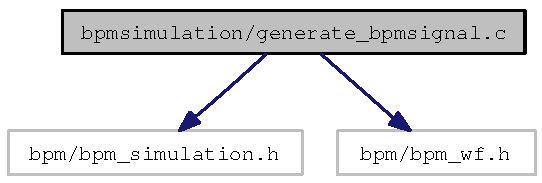
\includegraphics[width=148pt]{generate__bpmsignal_8c__incl}
\end{center}
\end{figure}
\subsubsection*{Functions}
\begin{CompactItemize}
\item 
int {\bf generate\_\-bpmsignal} ({\bf bpmconf\_\-t} $\ast$bpm, {\bf bpmmode\_\-t} $\ast$mode, {\bf beamconf\_\-t} $\ast$beam, {\bf doublewf\_\-t} $\ast$rf)
\end{CompactItemize}
